
% plantilla obtenida de: https://www.overleaf.com/19886281jjqffwsxshmm#/73112823/

\documentclass[a4paper, 11pt]{article}
\usepackage{comment} % enables the use of multi-line comments (\ifx \fi) 
\usepackage{lipsum} %This package just generates Lorem Ipsum filler text. 
\usepackage{fullpage} % changes the margin

\usepackage[spanish]{babel}
\usepackage[utf8]{inputenc}

\usepackage{graphicx}

\usepackage{amsmath}
\usepackage{amsfonts}
% or
\usepackage{amssymb}
\usepackage{tikz}
\usepackage{array}
\newcolumntype{C}{>{$}l<{$}} % math-mode version of "l" column type
\newcommand{\imageins}[4]{\begin{figure}[!ht]		%Take the hardwork from using images. Let this command do the work for you. Insert images by just using this command \imageins{filename}{width as a ratio of total text width of the page}{caption name}{label name for referring in articles}		
    \centering
    \includegraphics[width=#2\textwidth]{#1}
    %\caption{#3}
    %\label{#4}
    \vspace{0.2em}
\end{figure}}

%%%%%%%%%%%%%%%%%%%%%%%%%%%%%%%%%%%%%%%%%%%%%%%%%%%%%%%%%%%%%%%%%%%%%%%%%%%%%%%%%%
\usepackage{listings}
\usepackage{color}
 
\definecolor{codegreen}{rgb}{0,0.6,0}
\definecolor{codegray}{rgb}{0.5,0.5,0.5}
\definecolor{codepurple}{rgb}{0.58,0,0.82}
\definecolor{backcolour}{rgb}{0.95,0.95,0.92}
 
\lstdefinestyle{mystyle}{
    backgroundcolor=\color{backcolour},   
    commentstyle=\color{codegreen},
    keywordstyle=\color{magenta},
    numberstyle=\tiny\color{codegray},
    stringstyle=\color{codepurple},
    basicstyle=\footnotesize,
    breakatwhitespace=false,         
    breaklines=true,                 
    captionpos=b,                    
    keepspaces=true,                 
    numbers=left,                    
    numbersep=5pt,                  
    showspaces=false,                
    showstringspaces=false,
    showtabs=false,                  
    tabsize=2
}
 
\lstset{style=mystyle}

%%%%%%%%%%%%%%%%%%%%%%%%%%%%%%%%%%%%%%%%%%%%%%%%%%%%%%%%%%%%%%%%%%%%%%%%%%%%%%%%%%

\begin{document}
%Header-Make sure you update this information!!!!
\noindent
\large\textbf{Relación I} \hfill \textbf{Antonio Gámiz Delgado} \\
\normalsize Modelos de Computación \hfill 26/09/2018
%\normalsize ECE 100-003 \hfill Teammates: Student1, Student2 \\
%Prof. Oruklu \hfill Lab Date: XX/XX/XX \\
%TA: Adam Sumner \hfill Due Date: XX/XX/XX

\section*{Ejercicio 17}

Diseña un autómata finito determinista que reconozca el siguiente lenguaje:
\[
L_3=\{u\in\{0,1\}^*| \text{ el número de 1's no es múltiplo de 3 y el número de 0's es par }\}
\]

Primero realizamos el AFD que detecta las palabras que tienen un número de 1's que no es múltiplo de 3.

\begin{center}
\begin{tikzpicture}[scale=0.2]
\tikzstyle{every node}+=[inner sep=0pt]
\draw [black] (12.4,-16.4) circle (3);
\draw (12.4,-16.4) node {$q_0$};
\draw [black] (24.1,-16.3) circle (3);
\draw (24.1,-16.3) node {$q_1$};
\draw [black] (24.1,-16.3) circle (2.4);
\draw [black] (35.9,-16.3) circle (3);
\draw (35.9,-16.3) node {$q_2$};
\draw [black] (35.9,-16.3) circle (2.4);
\draw [black] (9.4,-16.4) -- (9.4,-16.4);
\fill [black] (9.4,-16.4) -- (8.6,-15.9) -- (8.6,-16.9);
\draw [black] (15.4,-16.37) -- (21.1,-16.33);
\fill [black] (21.1,-16.33) -- (20.3,-15.83) -- (20.3,-16.83);
\draw (18.25,-16.86) node [below] {$1$};
\draw [black] (27.1,-16.3) -- (32.9,-16.3);
\fill [black] (32.9,-16.3) -- (32.1,-15.8) -- (32.1,-16.8);
\draw (30,-16.8) node [below] {$1$};
\draw [black] (34.627,-19.008) arc (-32.11358:-147.3988:12.389);
\fill [black] (13.7,-19.1) -- (13.71,-20.04) -- (14.55,-19.5);
\draw (24.19,-25.32) node [below] {$1$};
\draw [black] (11.077,-13.72) arc (234:-54:2.25);
\draw (12.4,-9.15) node [above] {$0$};
\fill [black] (13.72,-13.72) -- (14.6,-13.37) -- (13.79,-12.78);
\draw [black] (22.777,-13.62) arc (234:-54:2.25);
\draw (24.1,-9.05) node [above] {$0$};
\fill [black] (25.42,-13.62) -- (26.3,-13.27) -- (25.49,-12.68);
\draw [black] (34.577,-13.62) arc (234:-54:2.25);
\draw (35.9,-9.05) node [above] {$0$};
\fill [black] (37.22,-13.62) -- (38.1,-13.27) -- (37.29,-12.68);
\end{tikzpicture}
\end{center}

Ahora hacemos el AFD que detecta las palabras con un número par de 0's:

\begin{center}
\begin{tikzpicture}[scale=0.2]
\tikzstyle{every node}+=[inner sep=0pt]
\draw [black] (14.6,-22.9) circle (3);
\draw (14.6,-22.9) node {$q_0$};
\draw [black] (14.6,-22.9) circle (2.4);
\draw [black] (25.7,-22.9) circle (3);
\draw (25.7,-22.9) node {$q_1$};
\draw [black] (11.5,-22.9) -- (11.6,-22.9);
\fill [black] (11.6,-22.9) -- (10.8,-22.4) -- (10.8,-23.4);
\draw [black] (17.123,-21.309) arc (111.72656:68.27344:8.176);
\fill [black] (23.18,-21.31) -- (22.62,-20.55) -- (22.25,-21.48);
\draw (20.15,-20.23) node [above] {$0$};
\draw [black] (13.277,-20.22) arc (234:-54:2.25);
\draw (14.6,-15.65) node [above] {$1$};
\fill [black] (15.92,-20.22) -- (16.8,-19.87) -- (15.99,-19.28);
\draw [black] (24.377,-20.22) arc (234:-54:2.25);
\draw (25.7,-15.65) node [above] {$1$};
\fill [black] (27.02,-20.22) -- (27.9,-19.87) -- (27.09,-19.28);
\draw [black] (23.767,-25.156) arc (-54.42218:-125.57782:6.216);
\fill [black] (16.53,-25.16) -- (16.89,-26.03) -- (17.47,-25.21);
\draw (20.15,-26.82) node [below] {$0$};
\end{tikzpicture}
\end{center}

Y ahora hacemos el producto de los dos:

\begin{center}
\begin{tikzpicture}[scale=0.2]
\tikzstyle{every node}+=[inner sep=0pt]
\draw [black] (11.3,-20.1) circle (3);
\draw (11.3,-20.1) node {$r_0$};
\draw [black] (25.4,-20.1) circle (3);
\draw (25.4,-20.1) node {$r_1$};
\draw [black] (25.4,-20.1) circle (2.4);
\draw [black] (41,-20.1) circle (3);
\draw (41,-20.1) node {$r_2$};
\draw [black] (41,-20.1) circle (2.4);
\draw [black] (55.3,-20.1) circle (3);
\draw (55.3,-20.1) node {$r_3$};
\draw [black] (11.3,-30.9) circle (3);
\draw (11.3,-30.9) node {$r_4$};
\draw [black] (25.4,-30.9) circle (3);
\draw (25.4,-30.9) node {$r_5$};
\draw [black] (14.3,-20.1) -- (22.4,-20.1);
\fill [black] (22.4,-20.1) -- (21.6,-19.6) -- (21.6,-20.6);
\draw (18.35,-20.6) node [below] {$1$};
\draw [black] (28.4,-20.1) -- (38,-20.1);
\fill [black] (38,-20.1) -- (37.2,-19.6) -- (37.2,-20.6);
\draw (33.2,-20.6) node [below] {$1$};
\draw [black] (42.091,-17.328) arc (146.66749:33.33251:7.252);
\fill [black] (42.09,-17.33) -- (42.95,-16.93) -- (42.11,-16.39);
\draw (48.15,-13.56) node [above] {$0$};
\draw [black] (13.74,-18.358) arc (121.86751:58.13249:23.506);
\fill [black] (13.74,-18.36) -- (14.68,-18.36) -- (14.16,-17.51);
\draw (26.15,-14.32) node [above] {$1$};
\draw [black] (44,-20.1) -- (52.3,-20.1);
\fill [black] (52.3,-20.1) -- (51.5,-19.6) -- (51.5,-20.6);
\draw (48.15,-20.6) node [below] {$0$};
\draw [black] (13.523,-22.069) arc (34.33432:-34.33432:6.083);
\fill [black] (13.52,-22.07) -- (13.56,-23.01) -- (14.39,-22.45);
\draw (15.08,-25.5) node [right] {$0$};
\draw [black] (27.333,-22.362) arc (27.75259:-27.75259:6.738);
\fill [black] (27.33,-22.36) -- (27.26,-23.3) -- (28.15,-22.84);
\draw (28.61,-25.5) node [right] {$0$};
\draw [black] (9.019,-29) arc (-144.15799:-215.84201:5.978);
\fill [black] (9.02,-29) -- (8.96,-28.06) -- (8.14,-28.64);
\draw (7.39,-25.5) node [left] {$0$};
\draw [black] (23.005,-29.149) arc (-140.99882:-219.00118:5.798);
\fill [black] (23.01,-29.15) -- (22.89,-28.21) -- (22.11,-28.84);
\draw (21.21,-25.5) node [left] {$0$};
\draw [black] (14.3,-30.9) -- (22.4,-30.9);
\fill [black] (22.4,-30.9) -- (21.6,-30.4) -- (21.6,-31.4);
\draw (18.35,-31.4) node [below] {$1$};
\draw [black] (52.873,-21.862) arc (-55.67241:-84.60775:52.089);
\fill [black] (52.87,-21.86) -- (51.93,-21.9) -- (52.49,-22.73);
\draw (42.12,-28.36) node [below] {$1$};
\draw [black] (53.946,-22.776) arc (-29.84506:-122.57321:28.602);
\fill [black] (13.74,-32.64) -- (14.14,-33.5) -- (14.68,-32.65);
\draw (36.66,-36.89) node [below] {$1$};
\draw [black] (7.9,-20.1) -- (8.3,-20.1);
\fill [black] (8.3,-20.1) -- (7.5,-19.6) -- (7.5,-20.6);
\end{tikzpicture}
\end{center}

\newpage

\section*{Ejercicio 22}

Dar una expresión regular para el lenguaje aceptado por el siguiente autómata:

\begin{center}
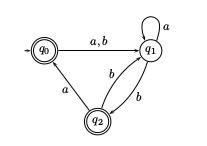
\includegraphics[scale=1]{./ej22.png}
\end{center}
\[
\left \{
  \begin{tabular}{CCCCCC}
  r^0_{00}&=\epsilon &\Longrightarrow r^1_{00}&=r^0_{00}+r^0_{00}(r^0_{00})^*r^0_{00}&=\epsilon+\epsilon(\epsilon)^*\epsilon&=\epsilon\\
  r^0_{01}&=a+b &\Longrightarrow r^1_{01}&=r^0_{01}+r^0_{00}(r^0_{00})^*r^0_{01}&=(a+b)+\epsilon(\epsilon)^*(a+b)&=a+b\\
  r^0_{02}&=\emptyset &\Longrightarrow r^1_{02}&=r^0_{02}+r^0_{00}(r^0_{00})^*r^0_{02}&=\emptyset+\epsilon(\epsilon)^*\emptyset&=\emptyset\\
  r^0_{10}&=\emptyset &\Longrightarrow r^1_{10}&=r^0_{10}+r^0_{10}(r^0_{00})^*r^0_{00}&=\emptyset+\emptyset(\epsilon)^*\epsilon&=\emptyset\\
  r^0_{11}&=a^+ &\Longrightarrow r^1_{11}&=r^0_{11}+r^0_{10}(r^0_{00})^*r^0_{01}&=a^++\emptyset(\epsilon)^*(a+b)&=a^+\\
  r^0_{12}&=b &\Longrightarrow r^1_{12}&=r^0_{12}+r^0_{10}(r^0_{00})^*r^0_{02}&=b+\emptyset(\epsilon)^*\emptyset&=b\\
  r^0_{20}&=a &\Longrightarrow r^1_{20}&=r^0_{20}+r^0_{20}(r^0_{00})^*r^0_{00}&=a+a(\epsilon)^*\epsilon&=a\\
  r^0_{21}&=b &\Longrightarrow r^1_{21}&=r^0_{21}+r^0_{20}(r^0_{00})^*r^0_{01}&=b+a(\epsilon)^*(a+b)&=b+a(a+b)\\
  r^0_{22}&=\emptyset &\Longrightarrow r^1_{22}&=r^0_{22}+r^0_{20}(r^0_{00})^*r^0_{02}&=\emptyset+a(\epsilon)^*\emptyset&=\emptyset
  
  \end{tabular}
  \right.
\]

\[
\left \{
	\begin{tabular}{CC}
r^2_{00}&= \epsilon\\
r^2_{01}&= a+b\\
r^2_{02}&= \emptyset\\
r^2_{10}&= \emptyset\\
r^2_{11}&= a^+\\
r^2_{12}&= b\\
r^2_{20}&= a\\
r^2_{21}&= b+a(a+b)\\
r^2_{22}&= \emptyset\\
	\end{tabular}
\right.
\]

Nos quedamos con:

\[
r^3_{12} + r^3_{32}=r^2_{01}+r^2_{02}(r^2_{22})^*r^2_{21}+r^2_{21}+r^2_{22}(r^2_{22})^*r^2_{21}=(a+b)+b+a(a+b) = a+b+a(a+b)
\]

\newpage

\section*{Ejercicio 23}

Sea $B_n=\{a^k | k \text{ es múltiplo de n }\}$. Demostrar que $B_n$ es regular para todo $n$.

\begin{center}
\begin{tikzpicture}[scale=0.2]
\tikzstyle{every node}+=[inner sep=0pt]
\draw [black] (10.3,-25.5) circle (3);
\draw (10.3,-25.5) node {$q_0$};
\draw [black] (10.3,-25.5) circle (2.4);
\draw [black] (21.9,-22) circle (3);
\draw (21.9,-22) node {$q_i$};
\draw [black] (34.4,-25.5) circle (3);
\draw (34.4,-25.5) node {$q_{n-1}$};
\draw [black] (6.7,-25.5) -- (7.3,-25.5);
\fill [black] (7.3,-25.5) -- (6.5,-25) -- (6.5,-26);
\draw [black] (11.813,-22.933) arc (137.97622:75.60344:7.47);
\fill [black] (19.22,-20.7) -- (18.57,-20.02) -- (18.32,-20.98);
\draw (14.41,-20.24) node [above] {$a$};
\draw [black] (24.601,-20.731) arc (104.85496:43.86055:8.339);
\fill [black] (32.75,-23.01) -- (32.56,-22.09) -- (31.84,-22.78);
\draw (29.74,-20.21) node [above] {$a$};
\draw [black] (32.137,-27.464) arc (-54.18653:-125.81347:16.726);
\fill [black] (12.56,-27.46) -- (12.92,-28.34) -- (13.5,-27.53);
\draw (22.35,-31.13) node [below] {$a$};
\end{tikzpicture}
\end{center}

El lenguaje $B_n$ es generado por este AFD, donde $i=1,...,n-2$, por lo tanto, $B_n$ es un lenguaje regular.

También se podría haber visto que es generado por la gramática de tipo 3 con lenguaje $\{a\}$ y las siguientes reglas de producción: $S \longrightarrow a^{k}S \quad | \quad \varepsilon$.

\section*{Ejercicio 24}

Decimos que $u$ es prefijo de $v$ si existe $w$ tal que $uw=v$. Decimos que $u$ es un prefijo propio de $v$ si además $u\neq v$ y $u\neq \varepsilon$. Demostrar que si $L$ es regular, también lo son los lenguajes

\begin{enumerate}
\item $NOPREFIJO(L)=\{u\in L | \text{ ningún prefijo propio de u pertenece a L }\}$

\item $NOEXTENSION(L)=\{u\in L | \text{ u no es un prefijo propio de ninguna palabra de L }\}$
\end{enumerate}
 
\section*{Ejercicio 25}

Si $L\subseteq A^*$, define la relación $\equiv$ en $A^*$ como sigue: si $u,v\in A^*$, entonces $u\equiv v $ si y solo si para toda $z\in A^*$, tenemos que ($uz\in L \Longleftrightarrow vz\in L$)

\begin{enumerate}
\item Demostrar que $equiv$ es una relación de equivalencia.

\begin{enumerate}
\item Reflexividad: Sea $z\in A^*$, si $uz\in L \Longleftrightarrow uz\in L$, luego $u\equiv u$.
\item Simetría: Si $u\equiv v \Longleftrightarrow (uz\in L \Longleftrightarrow vz\in L, \quad \forall z \in A^*) \Longleftrightarrow v\equiv u$.
\item Transitividad: Si $u\equiv y $ y $y\equiv v \Longleftrightarrow (uz\in L \Longleftrightarrow yz\in L, \quad \forall z \in A^*) \quad (yz\in L \Longleftrightarrow vz\in L, \quad \forall z \in A^*) \Longleftrightarrow u \equiv v$. 
\end{enumerate}

Por lo que la relación es reflexiva, simétrica y transitiva, por tanto, es una relación de equivalencia.

\item Calcular las clases de equivalencia de $L=\{a^ib^i|i\geq 0\}$.

Como las palabras de este lenguaje tienen el mismo número de a's que de b's, además de ser palíndromas, las palabras $u,v \in A^*$ que cumplan $uz\in L \Longleftrightarrow vz\in L, \quad \forall z \in A^*$ han de ser iguales, es decir, $u=v$.

Por lo que tenemos que el conjunto cociente es: $L/\equiv = \{[u] \quad | \quad u \in A^* \text{ y } [u]=u\}$

\item Calcular las clases de equivalencia de $L=\{a^ib^j|i,j\geq 0\}$.

Este apartado es diferente ya que no tenemos el problema de la simetría de la palabra.

Si $u=a^i \Longrightarrow [u] = \{v \in A^* \quad | \quad \text{ v es de la forma } v=a^j, \quad j \geq0\}$

Si $u=a^ib^j \Longrightarrow [u] = \{v \in A^* \quad | \quad \text{ v es de la forma } v=a^ib^j, \quad i,j \geq0\}$

\item Demostrar que $L$ es aceptado por un autómata finito determinístico si y solo si el número de clases de equivalencia es finito.

\item ¿Qué relación existe entre el número de clases de equivalencia y el autómata finito minimal que acepta $L$?

No sé cómo hacerlo, pero sospecho que el número de estados del AFM será igual al número de clases de equivalencia (por el apartado anterior).

\end{enumerate}

\end{document}